% 2D Image with indices
% Author: Peter Steinbach
\documentclass[tikz]{standalone}
%\documentclass[dvisvgm]{standalone}
%\def\pgfsysdriver{pgfsys-tex4ht.def}
\usepackage{units}
\usepackage{tikz}
\usetikzlibrary{calc,math,trees,positioning,arrows.meta,chains,shapes.geometric,shapes.arrows,%
    decorations.pathreplacing,decorations.pathmorphing,shapes,%
    matrix,shapes.symbols,fit,backgrounds}

 \pgfdeclarelayer{back}
 \pgfsetlayers{background,back,main}


\makeatletter
\makeatother

\begin{document}
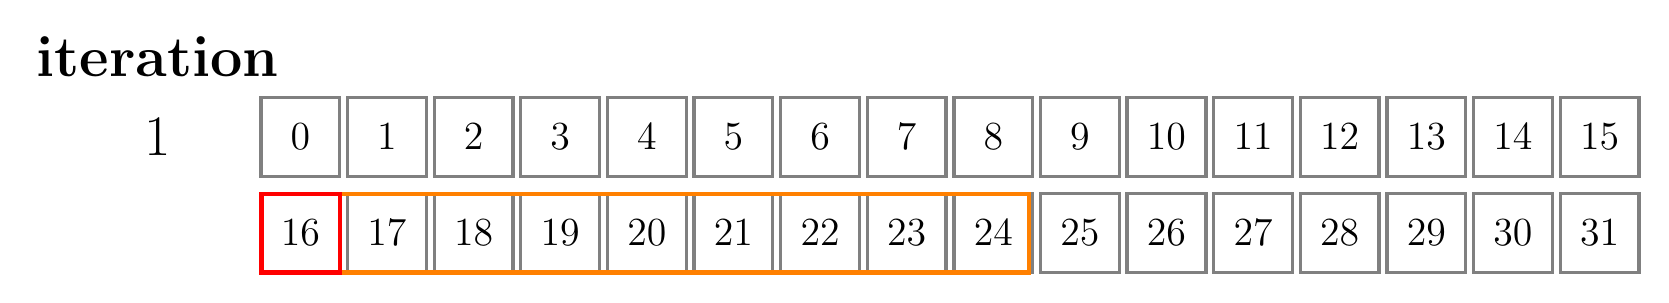
\begin{tikzpicture}

  \node (start) [draw=none,font=\huge,above] at(0,0) {\textbf{iteration}};
  \node (iter_0) [draw=none,font=\huge,above] at($(start.south)+(0,-1.)$) {$1$};
  

  \foreach \i in {0,...,15}
   {

     \tikzmath{
       integer \x;
       \x = \i+16;
     }

       \node (mem_\i) [rectangle,draw=gray,very thick,minimum width=1.cm,minimum height=1.cm,anchor=west,font=\Large] at($(iter_0.east)+(1.,0) + (1.1*\i,0)$) {$\i$};
       \node (mem_\x) [rectangle,draw=gray,very thick,minimum width=1.cm,minimum height=1.cm,font=\Large] at($(mem_\i.south) + (0,-.7)$) {$\x$};
     
     }
     
     \node (pref_0) [rectangle,draw=orange,ultra thick,minimum width=9.75cm,minimum height=1.cm,anchor=west] at($(mem_16.west)$) {};
     \node (acc_0) [rectangle,draw=red,ultra thick,minimum width=1.cm,minimum height=1.cm,anchor=west] at($(mem_16.west)$) {};

\end{tikzpicture}
\end{document}
